\newpage
\newsection{Setup}
\subsection{Installing Node.js}
Serverless Framework runs on Node v6 or higher so you have to install Node.js on your machine.
You can download it from this link: \url{https://nodejs.org/it/download/}
\begin{figure}[H]
		\centering
		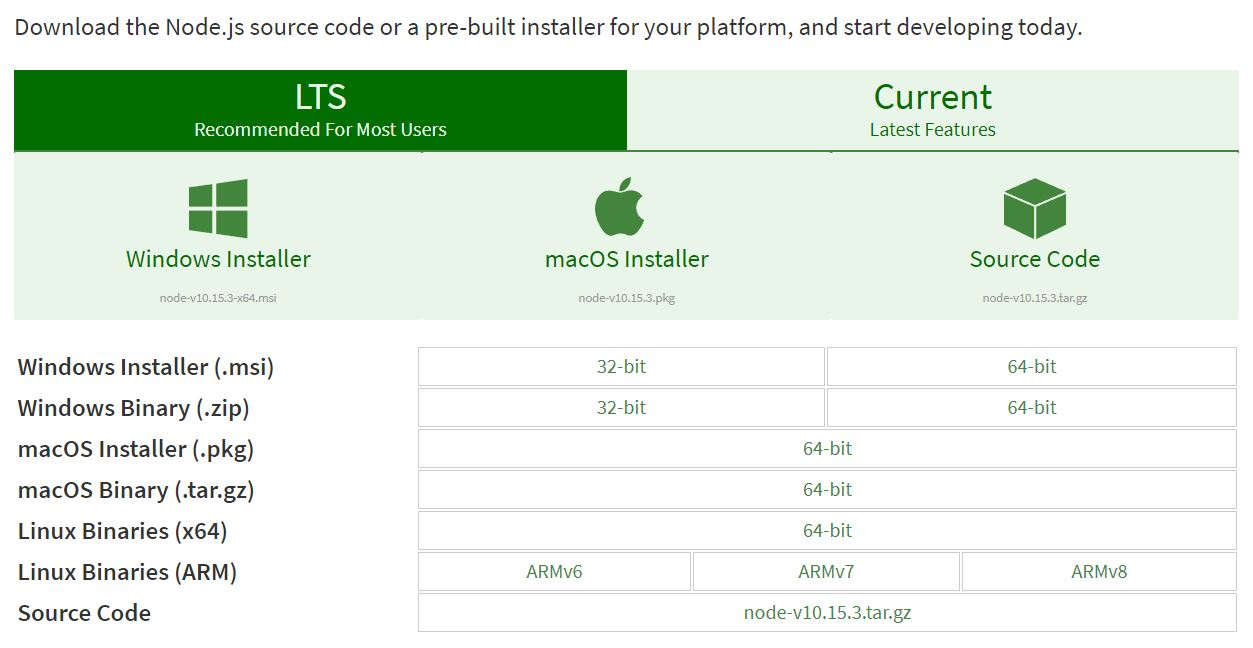
\includegraphics[scale=0.5]{../Img/node}
		\caption{Node.js download page}\label{}
\end{figure}
You can verify the correct installation running the commands:
\begin{ttfamily}node -v\end{ttfamily} and \begin{ttfamily}npm -v\end{ttfamily}
	
\subsection{Installing Serverless Framework}
You can install the Serverless Framework running the command:\begin{ttfamily} npm install -g serverless\end{ttfamily}
You can verify the correct installation of it running the command: \begin{ttfamily} serverless -v \end{ttfamily} or \\ \begin{ttfamily} sls -v\end{ttfamily}

\subsection{Setup AWS credentials}
You have to configure your serverless CLI with yours AWS credentials, so you have to create an IAM policy related with the Serverless Framework:
\begin{enumerate}
	\item Login to your AWS account and go to the Identity \& Access Management(IAM) page;
	\item Click on Users and then Add user;
	\item Enter a name in the first field to remind you this User is related to the Serverless Framework;
	\item Enable Programmatic access;
	\begin{figure}[H]
		\centering
		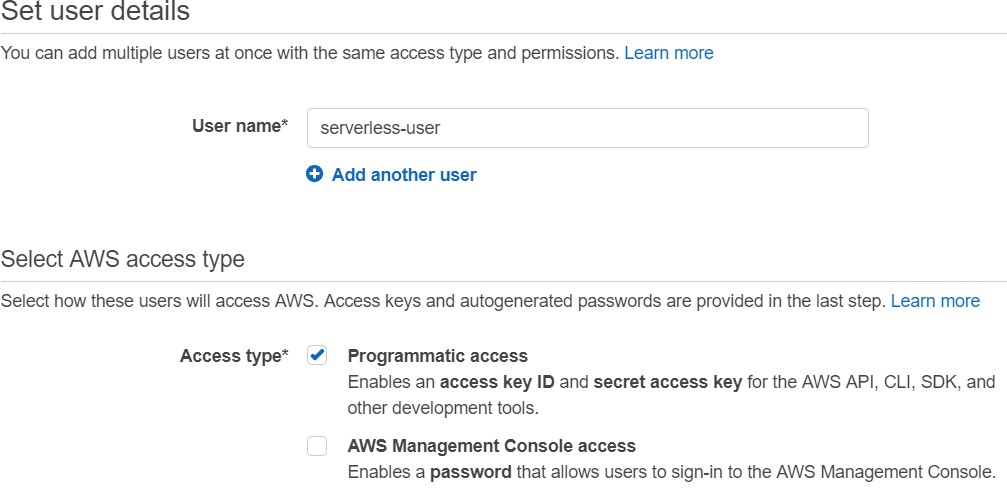
\includegraphics[scale=0.5]{../Img/setup1}
		\caption{Setup user details - AWS credentials}\label{}
	\end{figure}
	\item Click on Attach existing policies directly, search for and select \emph{AdministratorAccess};
	\begin{figure}[H]
		\centering
		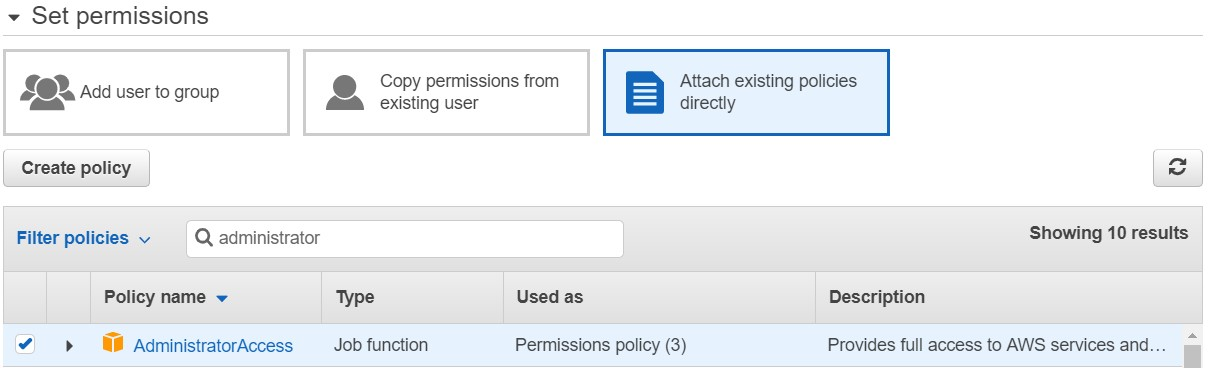
\includegraphics[scale=0.5]{../Img/setup2}
		\caption{Setup policy - AWS credentials}\label{}
	\end{figure}
	\item Create the user;
	\item Get the API key and secret;
	\item Run the command:
	\begin{ttfamily}serverless config credentials ---provider aws ---key YOURKEY ---secret YOURSECRET\end{ttfamily}
\end{enumerate}

\subsection{Deploying the serverless User Management service}
To deploy your serverless application you have to:
\begin{enumerate}
	\item Create a new directory;
	\item To create a new project run the command: \begin{ttfamily}serverless or sls\end{ttfamily}
	\item To install dependencies run the command: 
	\begin{ttfamily}npm install\end{ttfamily}
	\item To install a plugin you have to define it into the \emph{serverless.yml} and then run the command: 
	\begin{ttfamily}npm install -PLUGINNAME\end{ttfamily}
	\item To deploy your service run the command: 
	\begin{ttfamily}serverless deploy or sls deploy\end{ttfamily}
\end{enumerate}
